\documentclass[review]{vgtc}

\graphicspath{{figures/}{pictures/}{images/}{./}}

% Keep the VR template's metrics and line spacing; only add Unicode/CJK fonts.
\usepackage{times}
\renewcommand*\ttdefault{txtt}
\usepackage{mathptmx}

\usepackage{amsmath}
\usepackage{amssymb}
\usepackage{enumitem}
\hyphenation{Static-Lock Ego-Anchor}
\usepackage{array}
\usepackage{booktabs}
\usepackage{multirow}
\usepackage{tabularx}
\usepackage{xcolor}
\usepackage{placeins}

\onlineid{1118}
\vgtccategory{System}
\vgtcinsertpkg

\title{EgoAnchor: Zero-Shot Dynamic Anchoring of Everyday Objects in Passthrough Mixed Reality}

\author{%
  Hailin Ji 
  \thanks{e-mail: \texttt{jihailin@mail.bnu.edu.cn}} \\
  School of Artificial Intelligence \\
  Beijing Normal University \\
  Beijing, China
  \and Yifeng Chen 
  \thanks{e-mail: \texttt{yfchen@mail.bnu.edu.cn}} \\
  School of Artificial Intelligence \\
  Beijing Normal University \\
  Beijing, China
  \and Haonian Wang
  \thanks{e-mail: \texttt{haonianwang@mail.bnu.edu.cn}} \\
  School of Artificial Intelligence \\
  Beijing Normal University \\
  Beijing, China
  \and Yiran Zhang 
  \thanks{e-mail: \texttt{zhangyiran@mail.bnu.edu.cn}} \\
  School of Artificial Intelligence \\
  Beijing Normal University \\
  Beijing, China
  \and Hongwen Zhang 
  \thanks{Corresponding author; e-mail: \texttt{zhanghongwen@bnu.edu.cn}} \\
  School of Artificial Intelligence \\
  Beijing Normal University \\
  Beijing, China
  \and Yanhong Luo 
  \thanks{Corresponding author; e-mail: \texttt{273961431@xbmu.edu.cn}} \\
  College of Electrical Engineering \\
  Northwest Minzu University \\
  Lanzhou, China
}

\abstract{%
Zero-shot six-degree-of-freedom (6-DoF) object pose estimation enables the localization of unseen everyday objects. Its outputs, however, are asynchronous, low-rate, and variable in quality, making them unsuitable for direct use as continuous, stable object anchors in passthrough mixed reality (PMR). We present EgoAnchor, an egocentric system for zero-shot dynamic object anchoring. The perception backend produces camera-frame pose observations with visual-consistency scores. The runtime transforms these observations into world-frame object states at image capture time and maintains a reliable object state, thereby producing continuous, stable anchors with occlusion recovery. We implement EgoAnchor on Meta Quest 3 and evaluate it through controlled benchmarks using a platform-tracked controller reference, ablations of key components, and a within-subject study with 24 participants. Compared with the baselines, EgoAnchor reduces static registration error, occlusion-recovery error, and latency-aligned trajectory residuals, at the cost of longer motion-response latency. The user study also shows higher ratings for real--virtual integration, interaction trust, and willingness to rely on the system. The source code will be released upon acceptance.
}

\keywords{passthrough mixed reality, dynamic object anchoring, 6-DoF pose estimation, runtime system, user perception}

% ===== Teaser =====
\teaser{%
  \centering
  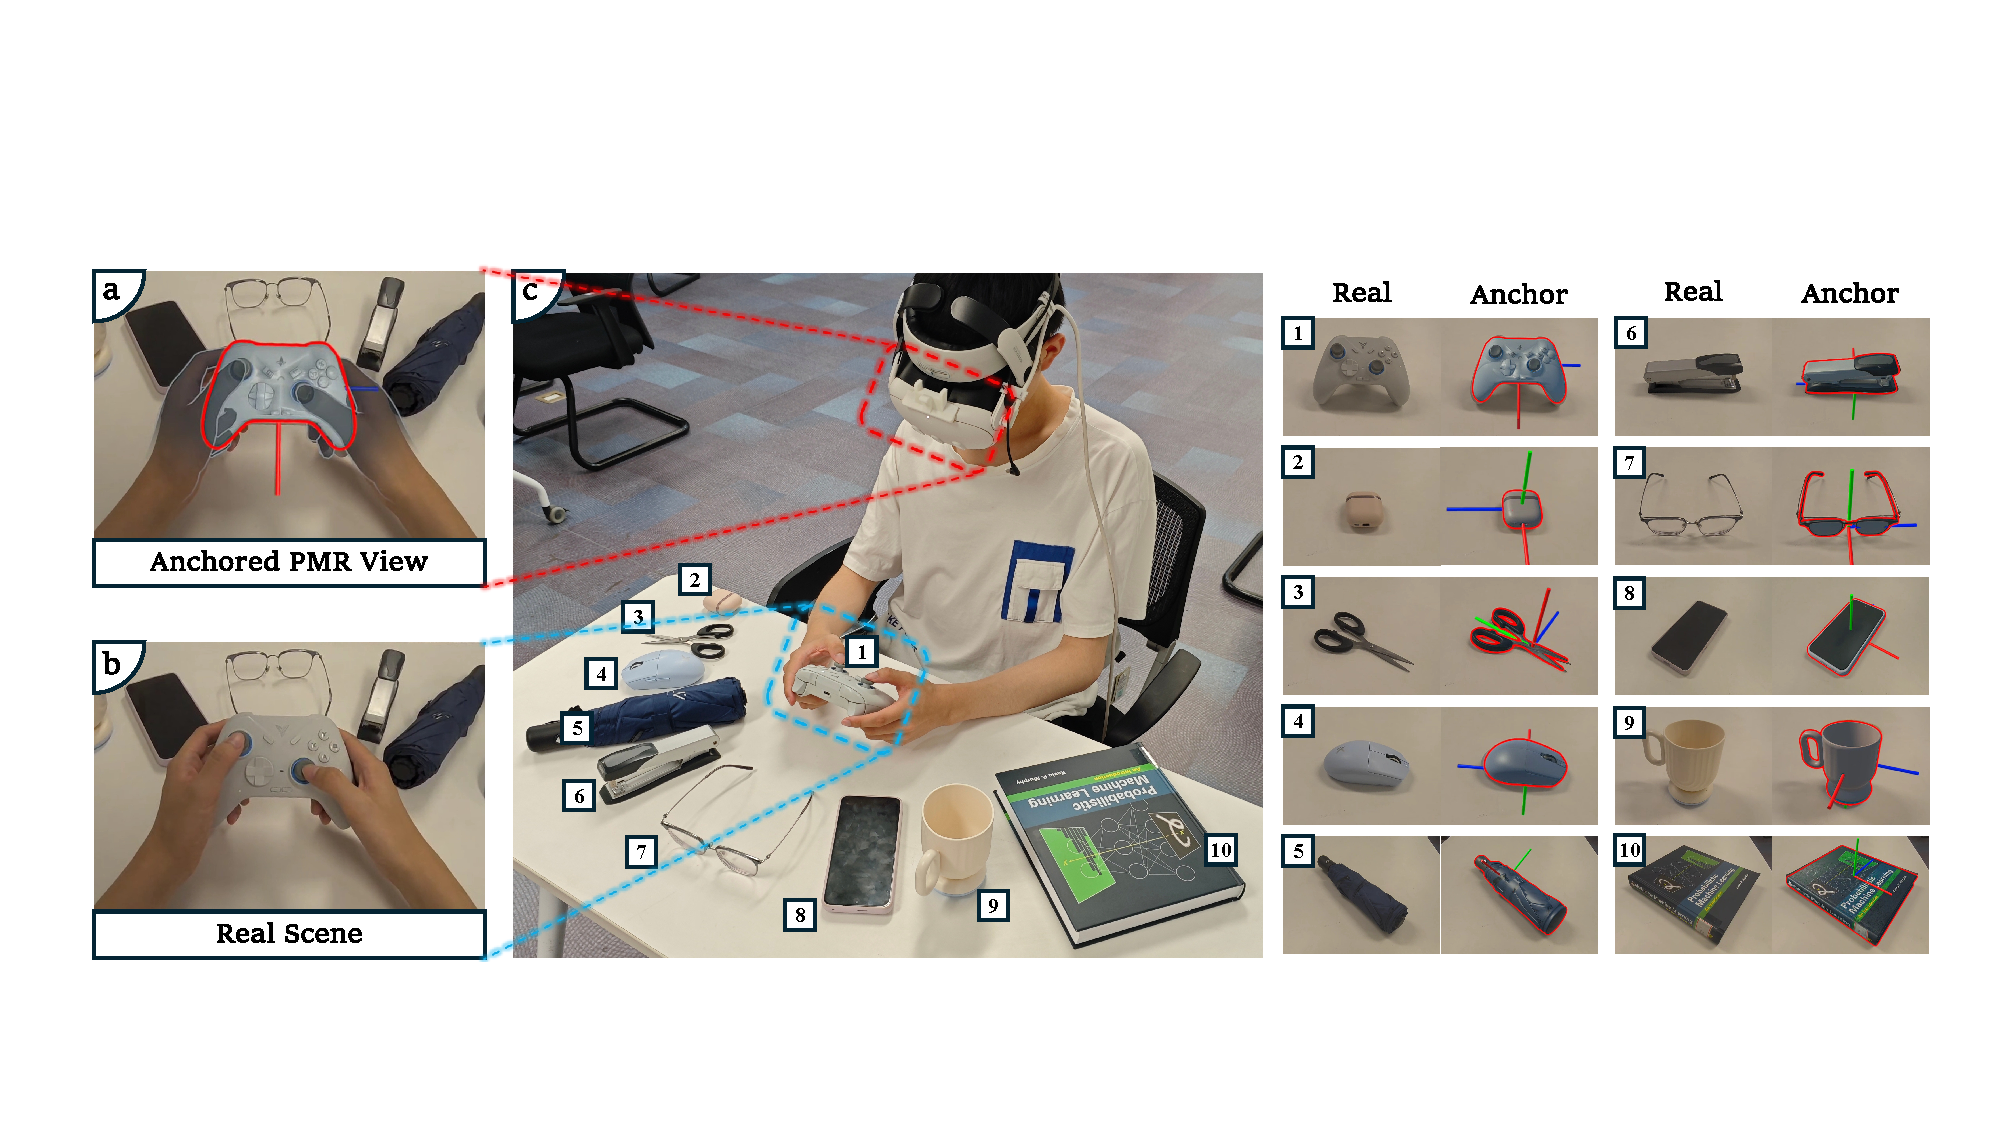
\includegraphics[width=\linewidth]{figures/teaser.pdf}
  \caption{Examples of zero-shot dynamic anchoring of everyday objects with EgoAnchor: (a) a first-person view with anchored augmentations; (b) the unaugmented passthrough view at the same time; and (c) a third-person view of the interaction. Scene numbers 1--10 correspond to the ten objects on the right; each group shows the physical object (Real) and the EgoAnchor visualization (Anchor). Red outlines and local coordinate axes indicate the estimated 6-DoF object anchors. The objects are, in order, a game controller, earbud case, scissors, wireless mouse, umbrella, stapler, eyeglasses, smartphone, mug, and book, covering varied scales, geometries, and appearances.}
  \label{fig:teaser}
}

\begin{document}

\firstsection{Introduction}\label{sec:introduction}
\maketitle

% ===== Problem motivation =====
Passthrough mixed reality (PMR) can attach virtual content to physical objects for operating instructions, interaction guidance, state visualization, and proximal interaction. Such applications must continuously maintain an object-level spatial state as the object moves: the virtual overlay should preserve a consistent six-degree-of-freedom (6-DoF) relationship with the object during head motion, object manipulation, and brief occlusion. Conventional spatial anchors target static environments and cannot represent the motion of individual objects. Dynamic object anchoring is therefore a fundamental capability for object-centered MR applications~\cite{selfblending2026,gradualreality2024}.

% ===== Limitations of existing solutions =====
Existing solutions provide partial support at different technical levels. Native object-tracking APIs on commercial headsets offer tight integration, but the supported object classes, geometric-model specifications, and runtime behavior are defined by the platform, as exemplified by Apple Vision Pro and Meta Quest. Fiducial markers such as AprilTag and ArUco, as well as dedicated hardware trackers such as the HTC Tracker, provide stable localization but require modifying the target object or attaching extra hardware. More recently, open-vocabulary detection, temporal segmentation, stereo matching, and model-based zero-shot 6-DoF pose estimation enable visual localization of rigid objects with known 3D models~\cite{groundingdino2025,cutie2024,fastfoundationstereo2026,foundationpose2024,gigapose2024}. These perception foundation models broaden the scope of visual localization, but their outputs remain discrete, asynchronous camera-frame pose observations tied to specific image-capture times. They therefore cannot directly provide reliable object anchors for MR rendering.

% ===== Core problem =====
Directly using visual pose estimates as object anchors introduces several challenges. First, an asynchronous estimate reaches the renderer only after nontrivial latency. Composing it with the headset pose at arrival time incorrectly attributes head motion to object motion. Second, pose candidates can fluctuate because of occlusion, depth noise, or geometric mismatch, and accepting them directly causes visible jitter. Finally, a noisy pose stream with a low and irregular update rate cannot match high-rate rendering. The runtime must also manage stationary and moving states, brief tracking failures, and reacquisition. A single-frame pose estimator is therefore insufficient for maintaining a continuously usable object anchor state.

% ===== EgoAnchor solution =====
We present EgoAnchor, an egocentric system for zero-shot dynamic object anchoring. The perception backend integrates open-vocabulary detection, temporal segmentation, stereo depth recovery, and zero-shot pose estimation into a continuous pipeline. It assesses each observation using a visibility-gated color--depth (VCD) reliability score. The runtime transforms asynchronous pose candidates into world-frame observations at capture time, maintains a temporal object state for real-time rendering, and produces continuously usable object anchors while the object moves, remains stationary, or is briefly unobserved. A new target requires only a 3D model and a short text description, with no fiducial marker or object-specific training. The 3D model can be an existing digital asset or reconstructed offline from images.

% ===== Contributions =====
Our main contributions are:
\begin{enumerate}[leftmargin=1.8em,itemsep=1pt,topsep=2pt]
  \item \textbf{EgoAnchor system:} We transform asynchronous, low-rate, and variable-quality zero-shot visual observations from the camera frame into continuously usable, world-frame dynamic object anchors.
  \item \textbf{Anchoring-aware perception and runtime:} VCD evaluates the reliability of each observation, while capture-time alignment, time-indexed trajectories, and static locking maintain continuous runtime output that recovers from tracking failures.
  \item \textbf{System evaluation:} Controlled benchmarks using a platform-tracked controller reference, ablations of key components, and a within-subject user study with 24 participants quantify system performance, design tradeoffs, and user perception.
\end{enumerate}

\section{Related Work}\label{sec:related-work}

\subsection{MR Object Anchoring}

Object anchoring establishes a spatial reference for a physical entity so that virtual content remains attached to and follows the object. Early methods estimate pose from fiducial markers such as AprilTag and ArUco~\cite{apriltag2011,aruco2014}. They require modifying the target object and do not readily extend to open-world settings.

Consumer MR platforms now offer markerless object recognition and tracking. Azure Object Anchors\footnote{\href{https://learn.microsoft.com/en-us/dynamics365/mixed-reality/guides/pc-app-anchor-object}{Azure Object Anchors}}, Vuforia Model Targets\footnote{\href{https://developer.vuforia.com/library/vuforia-engine/images-and-objects/model-targets/model-targets/}{Vuforia Model Targets}}, Apple Vision Pro\footnote{\href{https://developer.apple.com/documentation/visionos/implementing-object-tracking-in-your-app}{Apple object tracking}}, and Meta Quest\footnote{\href{https://developers.meta.com/horizon/documentation/native/android/mobile-dynamic-object-tracker/}{Meta dynamic object tracking}} establish object states using onboard sensing and target models. They typically depend on proprietary object scans or offline setup and are constrained by supported object types and platform interfaces. Research systems further combine headset tracking, spatial mapping, cameras, and depth sensing for asset localization, known-object registration, and continuous tracking~\cite{fan2021assettracking,doughty2022hmdegopose,pollabauer2023hololens,martingomez2024sttar,trojak2025mixedpose,greene2025markerless,trojak2026markerless,gbot2024}. However, they often rely on specific objects, task priors, dedicated hardware, or platform configuration, offering limited support for flexibly onboarding diverse everyday objects in open settings~\cite{hurt2025surrealitycv}.

\subsection{6-DoF Object Pose Estimation and Tracking}

6-DoF pose estimation recovers the camera-frame pose of a rigid object from visual observations and provides the perceptual basis for dynamic anchoring~\cite{aguirrezabal2026survey}. Research has progressed from local feature matching to known-instance estimation based on RGB-D fusion, dense geometric regression, symmetry modeling, and self-supervised learning~\cite{densefusion2019,epos2020,gdrnet2021,self6d2020}. It now extends to unseen objects and zero-shot settings~\cite{gen6d2022,megapose2022,lin2024sam6d,ornek2024foundpose,moon2025coop,foundationpose2024}, while particle filters and multi-frame geometric constraints maintain state across frames~\cite{poserbpf2021,bundletrack2021}.

Visual foundation models further broaden perception in open settings. Open-vocabulary detectors identify targets from natural-language descriptions~\cite{owlvit2022,glip2022,groundingdino2025,yoloe2025}; video object segmentation maintains identity and contours across frames~\cite{xmem2022,cutie2024}; and modern stereo matching improves depth recovery and cross-domain generalization in complex scenes~\cite{raftstereo2021,igevstereo2023,fastfoundationstereo2026}. Together, these advances make zero-shot localization of everyday objects increasingly practical, but they mainly address local perception in the camera frame. In MR, the observations must still be converted into stable and continuous world-frame object states.

\subsection{Temporal Alignment in XR}

Image capture, inference, and transmission in XR introduce end-to-end latency that varies over time, so the rendered state corresponds to an earlier observation~\cite{diluca2010latency,mrloop2022,stauffert2020mtp}. A common response to the mismatch between a state timestamp and the target display time is \emph{predictive tracking}: a motion model extrapolates historical states to the current or expected display time to reduce dynamic registration error~\cite{azuma1994improving,laviola2003double,pvt2023,yoon2022headmotion}.

An alternative retains timestamped state records and reconstructs a state by querying or interpolating at a past time. AR systems use timestamp synchronization, sampling adjustment, and interpolation or extrapolation to re-register data streams with different latencies~\cite{jacobs1997latency}. OpenXR\footnote{\href{https://registry.khronos.org/OpenXR/specs/1.1/man/html/xrLocateSpace.html}{OpenXR xrLocateSpace}} likewise distinguishes future-state prediction from a \emph{history query}: the former reduces phase lag, whereas the latter recovers spatial geometry at a past time.

\section{EgoAnchor System}\label{sec:system}

\subsection{System Overview}

EgoAnchor specifies a target using a text description and an offline 3D model, without fiducial markers or object-specific training. The perception backend produces a camera-frame pose with a reliability score. The runtime converts it into a world-frame pose at capture time and maintains the anchor on the rendering clock.

The runtime distinguishes the image-capture time $t_f$, candidate-arrival time $t_a$, and rendering time $t_r$. We use $T_a^b\in\mathrm{SE}(3)$ to denote a rigid transform from frame $a$ to frame $b$. The symbols $w$, $c$, and $o$ denote the world, left-camera, and local object frames, respectively; $\widehat{T}$ denotes a filtered state and $\widetilde{T}$ an application output. Fig.~\ref{fig:arch} shows the system architecture.

\begin{figure*}[t]
  \centering
  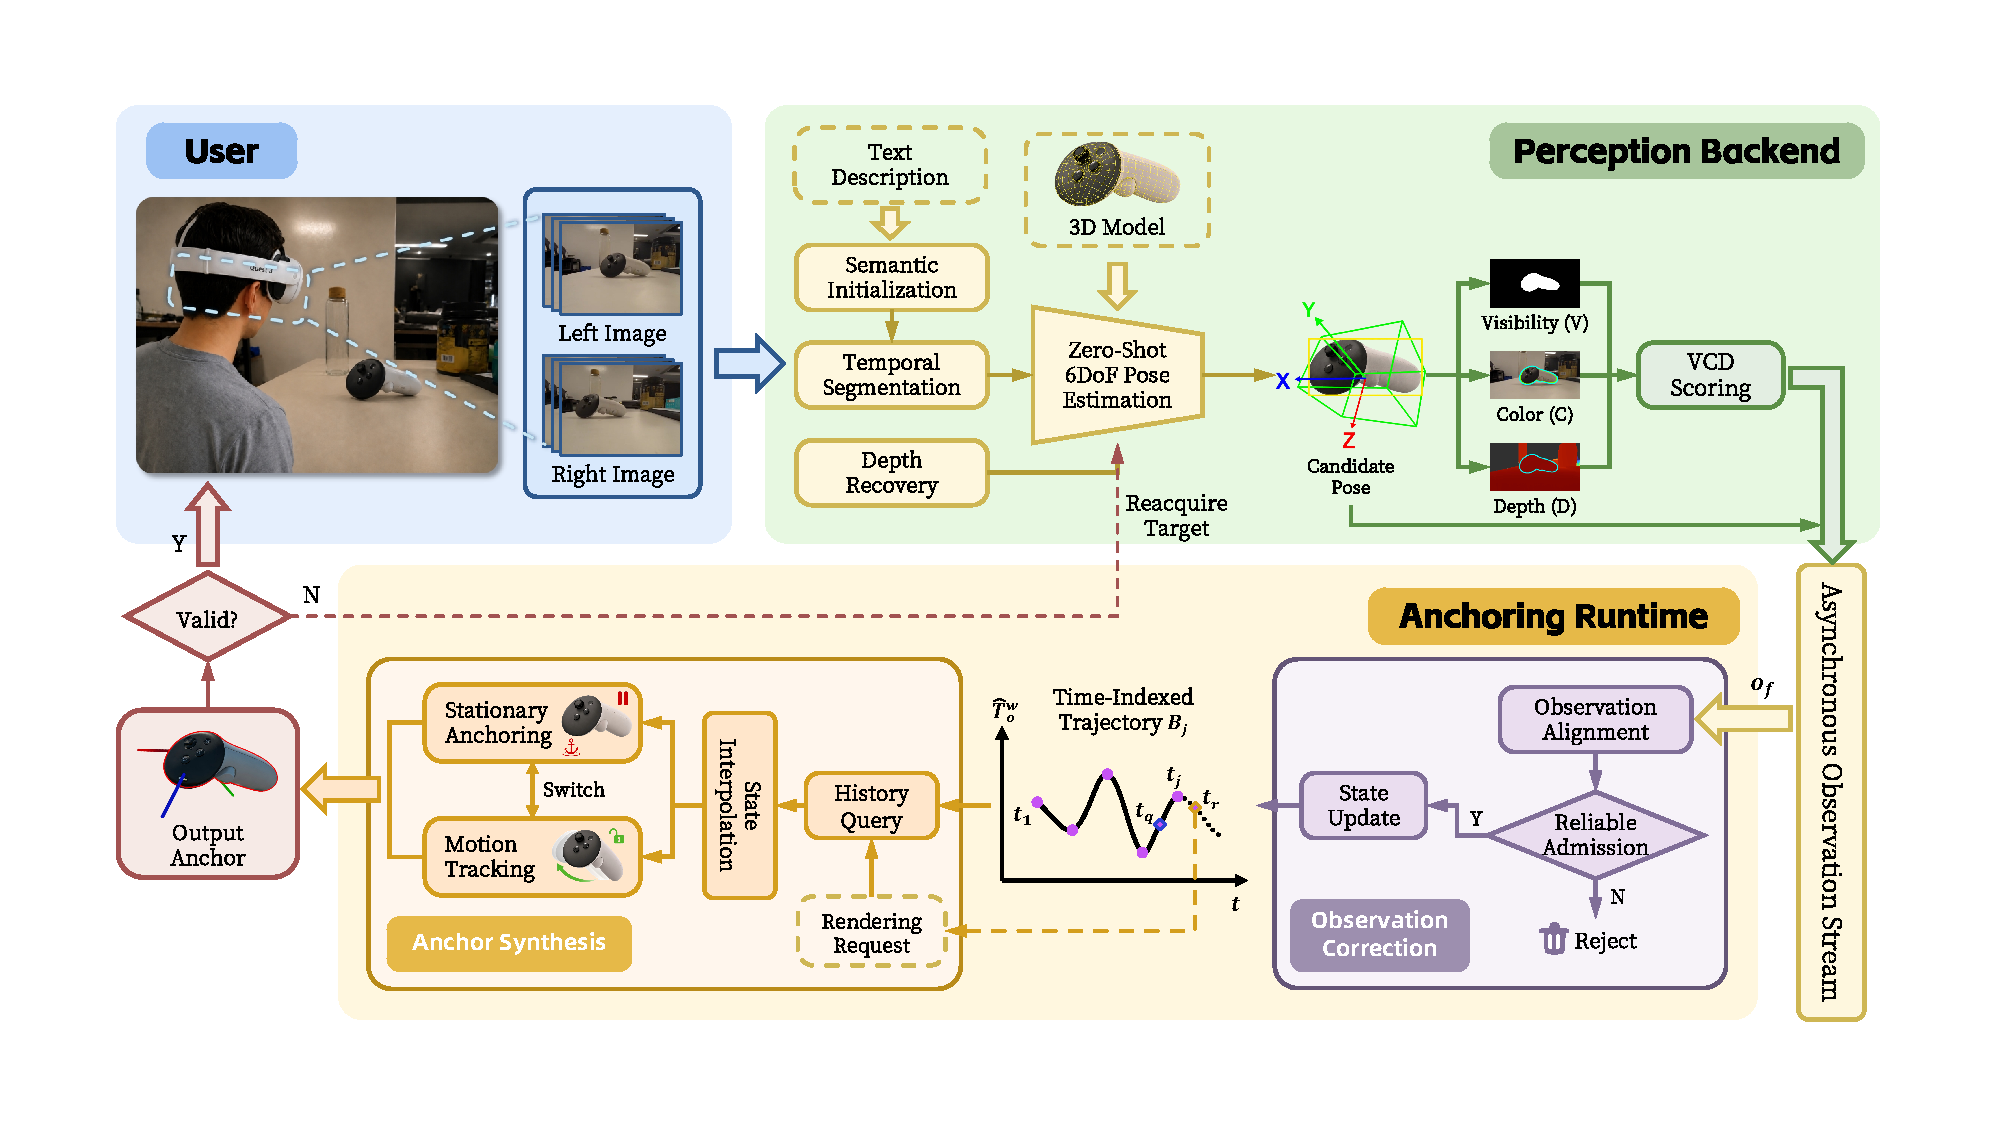
\includegraphics[width=\textwidth]{figures/pipeline_en.pdf}
  \caption{EgoAnchor architecture and asynchronous data flow. From stereo images, a text description, and a 3D model, the perception backend performs semantic initialization, temporal segmentation, depth recovery, and zero-shot 6-DoF pose estimation. It computes VCD reliability from visibility (V), color (C), and depth (D). When an asynchronous observation $o_f$ reaches the runtime, it is converted into a world-frame pose at capture time. Admission and state updates form a time-indexed trajectory $B_j$. At rendering time $t_r$, the runtime queries the trajectory at $t_q$ and switches between dynamic tracking and StaticLock. A sustained lack of reliable observations triggers reacquisition.}
  \label{fig:arch}
\end{figure*}

\subsection{Perception Backend}\label{sec:perception}

\textbf{Input and observation.}
Given stereo images $I_f = (I_f^L, I_f^R)$, a target description $Q_o$, and a 3D model $G_o$, the backend forms an observation for each processed frame:
\begin{equation}
o_f = (f, t_f, T_{o,f}^{c}, R_f),
\label{eq:observation}
\end{equation}
where $f$ is a monotonically increasing frame identifier, $T_{o,f}^{c}$ is the 6-DoF pose of the target in the left-camera frame, and $R_f \in [0,1]$ is the corresponding reliability score. The sequence $\{o_f\}$ forms an asynchronous observation stream.

\subsubsection{Anchoring-Oriented Perception Pipeline}

The pipeline establishes the target identity, metric depth, and camera-frame pose in sequence.

\textbf{Semantic initialization.}
At the initialization frame $f_0$, an open-vocabulary detector~\cite{yoloe2025} obtains the target segmentation mask from the left image and text description:
\begin{equation}
M_{f_0} = \operatorname{Detect}(I_{f_0}^{L}, Q_o),
\label{eq:detect}
\end{equation}
where $f_0$ is the first frame with both a valid mask and sufficient depth coverage. The system resets $f_0$ upon reacquisition.

\textbf{Temporal segmentation.}
The initial mask initializes a video object segmentation network~\cite{cutie2024}, which then propagates the temporal identity of the target frame by frame:
\begin{equation}
(M_f, H_f) = \operatorname{Seg}(I_f^{L}, H_{f-1}), \qquad f > f_0,
\label{eq:seg}
\end{equation}
where $H_f$ is the temporal appearance memory that maintains the identity of the target instance.

\textbf{Stereo depth recovery.}
A stereo matching network predicts disparity from rectified stereo images and recovers metric depth:
\begin{equation}
d_f = \operatorname{Stereo}(I_f^{L}, I_f^{R}), \qquad Z_f = \frac{b f_x}{d_f},
\label{eq:depth}
\end{equation}
where $b$ is the stereo baseline and $f_x$ is the focal length in pixels.

\textbf{Zero-shot 6-DoF pose estimation.}
A model-based estimator~\cite{foundationpose2024} recovers the camera-frame pose from the mask, depth, and 3D model:
\begin{equation}
T_{o,f}^{c} =
\begin{cases}
\operatorname{Reg}(M_f, Z_f, G_o), & \text{registration}, \\
\operatorname{Track}(M_f, Z_f, G_o, T_{o,f^-}^{c}), & \text{tracking}.
\end{cases}
\label{eq:pose}
\end{equation}
Global registration is used only for initialization and reacquisition; on subsequent frames, the previous result initializes local tracking.

\subsubsection{Per-Observation VCD Scoring}

Partial occlusion or noise can make a zero-shot pose candidate inconsistent with the image evidence. VCD compares a rendering against the corresponding observation~\cite{deepim2018,latentfusion2020,focalpose2022} and combines visibility (V), color (C), and depth (D) to assess candidate reliability.

\textbf{Visibility gating.}
Let $M_f^{\mathrm{rnd}}$ be the mask rendered at the candidate pose. We define:
\begin{equation}
\Omega_f = M_f \cap M_f^{\mathrm{rnd}}, \quad \Omega_f^{\circ} = \operatorname{Erode}(\Omega_f), \quad V_f = \frac{|\Omega_f|}{|M_f^{\mathrm{rnd}}|},
\label{eq:visibility}
\end{equation}
where $V_f$ is the fraction of the rendered projection supported by the observed mask. The eroded region $\Omega_f^\circ$ reduces the effect of mixed pixels near object boundaries.

\textbf{Color and depth consistency.}
Color consistency $S_f^C$ uses zero-mean normalized cross-correlation (ZNCC) in the CIE $L^*a^*b^*$ color space, with a lower weight for the lightness channel. Depth consistency combines a distance-adaptive absolute-residual term $S_f^{D,\mathrm{abs}}$ with a surface-normal structural term $S_f^{D,\mathrm{str}}$ that is robust to global depth bias:
\begin{equation}
S_f^D = (1-\alpha_f)\,S_f^{D,\mathrm{abs}} + \alpha_f\,S_f^{D,\mathrm{str}}.
\label{eq:depth-score}
\end{equation}
The local depth variation determines $\alpha_f$, emphasizing absolute depth for flat targets and local structure for targets with greater geometric variation.

\textbf{Evidence aggregation.}
Let $K_f\subseteq\{C,D\}$ be the set of valid modalities in the current frame. The combined score is:
\begin{equation}
R_f = V_f \cdot
\begin{cases}
\exp\!\left(\dfrac{\sum_{k \in K_f} w_k \ln \max(S_f^{k}, \epsilon)}{\sum_{k \in K_f} w_k}\right), & K_f \neq \varnothing, \\[6pt]
1, & K_f = \varnothing,
\end{cases}
\label{eq:vcd}
\end{equation}
where $w_k$ is the modality weight and $\epsilon$ prevents a logarithmic singularity. Invalid modalities are excluded from aggregation. If neither color nor depth is available, the score reduces to $V_f$. The multiplicative gate directly lowers reliability under severe occlusion or projection misalignment.

\subsection{Anchoring Runtime}\label{sec:anchoring}

The runtime converts low-rate asynchronous pose candidates into display-synchronous object states for rendering. On arrival, a candidate is transformed into a world-frame pose at capture time and used to update the trajectory. Rendering frames synthesize anchors by interpolation and manage StaticLock and validity. Decoupling candidate and rendering events prevents the inference rate from limiting the output rate.

\subsubsection{Observation Correction}\label{sec:obs-update}

The runtime transforms each candidate into a world-frame pose at capture time, then updates the trajectory after reliability and temporal admission checks.

\textbf{Observation alignment.}
Candidate $T_{o,f}^{c}$ corresponds to capture time $t_f$ but arrives at $t_a$. Composing it with the camera pose at arrival time introduces the intervening head motion into the object pose. The runtime retrieves the cached $T_{c,f}^{w}$ using frame identifier $f$ and computes:
\begin{equation}
T_{o,f}^{w} = T_{c,f}^{w}
\begin{bmatrix}
1 & 0 & 0 & 0 \\
0 & -1 & 0 & 0 \\
0 & 0 & 1 & 0 \\
0 & 0 & 0 & 1
\end{bmatrix}
T_{o,f}^{c}
\begin{bmatrix}
-1 & 0 & 0 & 0 \\
0 & 1 & 0 & 0 \\
0 & 0 & 1 & 0 \\
0 & 0 & 0 & 1
\end{bmatrix}.
\label{eq:capture-alignment}
\end{equation}
The two fixed matrices account for differences among the axis conventions of the vision, rendering, and local object coordinate systems.

\textbf{Reliability-based admission.}
Let $(t_j,T_{o,j}^{w},R_j)$ denote the $j$th admitted observation. The first candidate establishes a trajectory once it meets the reliability threshold; subsequent candidates must also have increasing timestamps:
\begin{equation}
R_f \geq R_{\min}, \qquad t_f > t_j \quad (j \geq 1).
\label{eq:admission}
\end{equation}
Candidates that fail these admission conditions do not update the internal state.

\textbf{State update.}
Each admitted observation updates constant-velocity Kalman filters~\cite{kalman1960new} for translation and rotation, producing the smoothed state $\widehat{T}_{o,j}^{w}$ and a time-indexed trajectory:
\begin{equation}
B_j = \{(t_i, \widehat{T}_{o,i}^{w})\}_{i=1}^{j}.
\label{eq:trajectory}
\end{equation}
The update also refreshes the motion and reliability measures used for StaticLock.

\subsubsection{Anchor Synthesis}\label{sec:frame-output}

Trajectory $B_j$ has a low and irregular update rate. The runtime first determines the history-query time $t_q$ and then interpolates adjacent nodes to generate a per-frame state.

\textbf{History query.}
The age of the latest available node at time $t_j$ relative to rendering time $t_r$ is $\ell_r=t_r-t_j$. The runtime dynamically sets the query lag from its estimate $\bar{\ell}_r$, obtained by asymmetric exponential smoothing:
\begin{equation}
\ell_r = t_r - t_j, \qquad \Delta_r = \max(\Delta_{\min},\, s\,\bar{\ell}_r), \qquad t_q = t_r - \Delta_r.
\label{eq:target-time}
\end{equation}
Here, $\Delta_{\min}$ is the minimum query lag and $s$ is a scale factor. This strategy increases the probability that $t_q$ falls between two nodes that have already arrived.

\textbf{State interpolation.}
When $t_i\leq t_q\leq t_{i+1}$, the runtime geometrically interpolates the object pose between adjacent trajectory nodes:
\begin{equation}
\lambda_q = \frac{t_q - t_i}{t_{i+1} - t_i}, \qquad
\widehat{T}_o^w(t_q) = \operatorname{Interp}(\widehat{T}_{o,i}^{w}, \widehat{T}_{o,i+1}^{w}; \lambda_q).
\label{eq:history-interp}
\end{equation}
Position uses linear interpolation (LERP), and rotation uses quaternion spherical linear interpolation (SLERP). Outside the trajectory interval, the nearest endpoint state is held.

\textbf{Output mode.}
To suppress small fluctuations while the object is stationary, EgoAnchor adaptively switches between dynamic tracking and StaticLock:
\begin{equation}
\widetilde{T}_o^w(t_r) = \begin{cases}
\widehat{T}_o^w(t_q), & \text{tracking}, \\
T_{o,\mathrm{lock}}^w, & \text{locked}.
\end{cases}
\label{eq:staticlock}
\end{equation}

\subsubsection{Static Locking}\label{sec:staticlock}

We introduce StaticLock, a static-state anchoring mechanism that switches to a locked pose when motion remains low and observations are reliable, then smoothly releases the lock when clear motion or reduced reliability is detected.

\textbf{Entry.}
The translation and rotation rates $\bar v_j$ and $\bar\omega_j$ are computed from consecutive admitted observations and exponentially smoothed. We define the joint condition:
\begin{equation}
\max\left(\frac{\bar{v}_j}{v_{\mathrm{th}}},\ \frac{\bar{\omega}_j}{\omega_{\mathrm{th}}}\right) \leq 1, \qquad R_j \geq R_{\mathrm{lock}}.
\label{eq:lock-entry}
\end{equation}
Once the condition holds for $\tau_{\mathrm{dwell}}$, the current tracked pose initializes $T_{o,\mathrm{lock}}^w$, and the low-pass-filtered reference pose $T_{o,\mathrm{ref}}^w$ is frozen to measure accumulated drift.

\textbf{Locked-state update.}
Let $d_{p,j}$ and $d_{\theta,j}$ denote the translation and rotation residuals between the current observation and the locked pose. Using deadband thresholds $d_{\mathrm{db}}$ and $\theta_{\mathrm{db}}$, we define the normalized deviation $\delta_j=\max(d_{p,j}/d_{\mathrm{db}},d_{\theta,j}/\theta_{\mathrm{db}})$. The locked pose is updated as:
\begin{equation}
T_{o,\mathrm{lock},j}^w =
\begin{cases}
\operatorname{Interp}\left(T_{o,\mathrm{lock},j-1}^w, T_{o,j}^{w};\, g_j\right), & \delta_j \leq 1, \\
T_{o,\mathrm{lock},j-1}^w, & \delta_j > 1.
\end{cases}
\label{eq:lock-update}
\end{equation}
Here, $g_j$ is a small gain modulated by reliability. The damped update absorbs drift within the deadband, whereas deviations outside it contribute to unlocking.

\textbf{Release.}
The system smoothly returns to tracking mode on the next rendering frame when a residual outside the deadband persists, drift relative to $T_{o,\mathrm{ref}}^w$ exceeds its limit, clear sustained motion is detected, or reliability drops sharply. The motion criterion is moderately relaxed as head-motion intensity increases to reduce false releases.

\textbf{Validity and reacquisition.}\label{sec:validity}
Recent reliable observations determine whether an anchor is marked valid, uncertain, or lost. During a brief observation gap, the runtime continues to query the trajectory and may hold the last trusted pose; after a timeout, it stops output. When an anchor is lost or candidates remain unreliable, the backend repeats detection and registration and resets the trajectory. The first newly admitted observation begins a new tracking cycle.

\section{System Implementation}\label{sec:implementation}

The EgoAnchor backend and runtime communicate over a local network. The perception backend runs on a workstation with an NVIDIA RTX 5090 GPU and uses Python 3.14.6, PyTorch 2.12.1, CUDA 13.2, and TensorRT 11.1. The client runtime is built with Unity 6000.3.11f1 and Meta XR SDK 203.0.0 and runs through Quest Link on a host with an Intel i9-14900K processor and 32~GB of memory. Meta Quest 3 provides stereo passthrough capture, device tracking, and rendering.

\textbf{Perception backend.}
The backend uses YOLOE-26 to initialize the open-vocabulary target~\cite{yoloe2025}, Cutie to propagate the target mask~\cite{cutie2024}, Fast-FoundationStereo to recover metric depth~\cite{fastfoundationstereo2026}, and FoundationPose for zero-shot 6-DoF registration and local tracking~\cite{foundationpose2024}. VCD uses nvdiffrast for hardware-accelerated online model rasterization~\cite{nvdiffrast2020}. On the RTX 5090 configuration, the median and P95 server-side processing times during tracking are 75.44~ms and 88.47~ms, respectively, and the median candidate-arrival rate is 13.25~Hz. All subsequent quantitative experiments use this hardware configuration.

\textbf{Anchoring runtime.}
The runtime is implemented in C\#. It obtains rectified stereo images and camera calibration parameters through the Meta Passthrough Camera API and caches a camera-pose history indexed by frame identifier. All runtime thresholds and gain parameters remain fixed across the three evaluation experiments; the complete parameter list is included in the supplemental material.

\textbf{Communication.}
Stereo images and camera calibration data are transmitted through ZeroMQ and Protobuf using a latest-frame-first policy to prevent queue buildup. The 6-DoF poses, system states, and control signals are transmitted over a NATS Core message bus. Image frames and returned observations retain the same frame identifier, allowing the runtime to retrieve the camera pose at the corresponding capture time.

\section{Evaluation Design}\label{sec:evaluation}

We evaluate EgoAnchor through three complementary experiments. Experiment~1 compares the static, dynamic, and state-transition behavior of four runtime configurations under controlled conditions. Experiment~2 examines capture-time alignment, static locking, VCD reliability ranking, and predictive tracking versus history query. Experiment~3 uses a within-subject study with 24 participants and everyday rigid objects to examine perceived anchoring quality, real--virtual integration, interaction trust, and willingness to rely on the system.

The 3D models of everyday objects are generated from multi-view smartphone photographs using Hunyuan3D\footnote{\url{https://3d.hunyuan.tencent.com/}}~\cite{hunyuan3d22025tencent}, followed by mesh simplification and texture baking. The Quest 3 controller uses the official standard digital asset.

\subsection{Experiment 1: System Performance}\label{sec:exp1-design}

\textbf{Reference and scenarios.}
The evaluation uses a Quest 3 controller as the visual tracking target and the 6-DoF pose reported by the platform SDK as the tracking reference. Four capture scenarios cover active head motion around a stationary target, start--stop transitions between rest and 6-DoF motion, continuous spatial translation and rotation, and tracking recovery after complete occlusion. These scenarios assess static stability, state-transition response, dynamic following, and occlusion-recovery performance, respectively.

\textbf{Conditions.}
All four configurations receive the same raw pose-candidate stream. \textbf{Arrival} and \textbf{Capture} both hold the latest candidate but use the camera pose at arrival time and capture time, respectively, when transforming it into the world frame. \textbf{One-Euro}~\cite{casiez2012oneeuro} is a representative smoothing baseline that balances jitter suppression and low-latency response in real-time interactive systems. It applies a speed-adaptive low-pass filter to admitted observations and maintains a time-indexed trajectory, but does not use StaticLock. \textbf{EgoAnchor} is the complete system.

\textbf{Metrics.}
Nine quantitative metrics are divided into three groups according to system response. \textbf{Static registration} includes head-motion coupling error (the spatial anchor displacement induced by observer head motion around a stationary target), registration error (the spatial deviation from the platform tracking reference), and static jitter (the pose change between consecutive rendering frames while the target is stationary). \textbf{Dynamic following} includes effective latency (the temporal offset that minimizes the residual between estimated and reference trajectories), LA-RMSE (the geometric trajectory residual after latency alignment), CT-RMSE (the current-time error without latency alignment), and residual jitter (the high-frequency component of the residual after latency alignment). \textbf{State-transition response} includes occlusion-recovery error (the pose deviation from the onset of occlusion until tracking restabilizes) and motion-response latency (the interval from the onset of object motion until the anchor begins to respond). All metrics are reported separately for translation and rotation, except motion-response latency, which is a scalar statistic shared across channels.

\subsection{Experiment 2: Ablation Analysis}\label{sec:exp2-design}

Experiment~2 ablates four key design choices.

\textbf{Observation alignment.}
The same camera-frame candidates are composed with the camera poses at image capture time and candidate-arrival time. We compare head-motion coupling error under active head motion to assess how capture-time alignment affects static registration.

\textbf{Static locking.}
We disable StaticLock in the complete EgoAnchor system and compare head-motion coupling error and jitter under stationary conditions, thereby quantifying the contribution of the module to anchor stability while the object is at rest.

\textbf{VCD.}
We rank candidates by decreasing VCD score, plot risk--coverage curves, and use the area under the risk--coverage curve (AURC) to quantify how well the score ranks geometric error~\cite{riskcontrolled2020,ding2020uncertainty}. A lower AURC indicates that higher-scoring candidates generally have lower geometric error.

\textbf{Prediction versus history query.}
To quantify the tradeoff between response speed and trajectory fidelity, we compare \emph{predictive tracking} with \emph{history query}. Predictive tracking extrapolates a Kalman-filtered constant-velocity model to $t_r$. History query follows Sec.~\ref{sec:frame-output}, applying translation LERP and rotation SLERP to adjacent trajectory nodes at $t_q$. Both methods share the same candidate stream, state estimation, and admission rules.

\subsection{Experiment 3: User Study}\label{sec:exp3-design}

Experiment~3 examines whether the system differences in the controlled evaluation are reflected in user perception. We compare One-Euro with the complete EgoAnchor system on everyday rigid objects, focusing on static stability, attachment during motion, occlusion recovery, perceived real--virtual integration, interaction trust, and willingness to rely on the anchor.

\subsubsection{Study Design}

The study used a wireless mouse, stapler, and game controller, which have complementary visual observability and manipulation-occlusion characteristics. They represent a weakly textured curved surface; an elongated, multi-planar shape; and an object with rich geometry and texture that is readily occluded by a natural grasp. We used a fully within-subject design. Each participant experienced One-Euro and EgoAnchor with all three objects. The six method--object conditions were ordered using a balanced Latin square and presented under anonymous A/B labels to reduce order effects.

\subsubsection{Tasks}

For each method--object condition, participants performed three standardized operations in order: (1) observing the stationary object from multiple angles; (2) picking up the object, translating it by approximately 25--30~cm, rotating it naturally by 30--45$^\circ$, and then returning it to its initial location; and (3) completely occluding the target with a standard panel for approximately 1~s, removing the panel, and observing recovery. Participants completed the subjective scales after the three tasks.

\subsubsection{Subjective Measures}

Subjective measures include seven object-anchoring items and three standardized scales: Augmentation Quality (AQ), Trust in Automation (TiA), and S-TIAS.

\textbf{Object-anchoring items.}
Seven items use a seven-point agreement scale and cover the application-level behaviors examined in Experiment~1, informed by prior work on AR tracking and trust~\cite{trustar2024}. Phase-specific behaviors include static stability, attachment during motion, pose consistency, and recovery consistency. Overall judgments include positional correctness, willingness to rely on the system, and the stability--responsiveness tradeoff. Each item is analyzed separately; the full wording appears in the supplemental material.

\textbf{Augmentation Quality (AQ).}
We use the full three-item Embedding Quality (EQ) and Interaction Quality (IQ) subscales of AQ~\cite{aq2026}. They assess real--virtual integration (geometric embedding) and interaction quality during manipulation, respectively, on seven-point scales.

\textbf{User trust (TiA and S-TIAS).}
TiA~\cite{tia2019} uses the Reliability/Competence (six items) and Understanding/Predictability (four items) subscales on five-point scales. S-TIAS~\cite{stias2025} measures overall interaction trust using three seven-point items. We adapt only the referent of each item to the study context. The Chinese translations were checked item by item and pilot-tested for comprehensibility.

The final questionnaire separately records overall method preference, trust choice, preference strength, confidence in distinguishing the methods, and post-study discomfort. These outcomes are reported descriptively.

\subsubsection{Procedure}

The study received approval from the institutional ethics review board. Participants provided written informed consent before the experiment. After a background survey, headset fitting, and task practice, participants completed the six method--object conditions in sequence and answered the object-anchoring items and AQ scale after each condition. After all conditions, they rated both methods using TiA and S-TIAS and completed the final questionnaire. Each session lasted approximately 60 minutes, with breaks available as needed.

\subsubsection{Participants}

The study included 24 participants, all of whom were retained in the final analysis (age 20--36 years, $M=27.08$, $\mathrm{SD}=4.45$; 12 women and 12 men; 22 right-handed). Six had never used VR/MR, 10 had used it 1--5 times, and eight had used it more than six times. Twelve had no prior experience with spatial manipulation of physical objects in AR/MR.

\subsubsection{Statistical Analysis}

For each participant, we first averaged each of the seven object-anchoring item scores and the two AQ subscale scores across the three objects. We separately averaged the items in the two TiA subscales and S-TIAS for each method, yielding 12 outcomes. For each measure, we report the median and interquartile range, $\mathrm{Mdn}\ [\mathrm{Q}_1, \mathrm{Q}_3]$. We tested the 24 paired samples using two-sided Wilcoxon signed-rank tests and report the paired rank-biserial correlation $r_{\mathrm{rb}}$ with its 95\% confidence interval. The seven custom items and five standardized-scale outcomes form two separate Holm--Bonferroni correction families. Cronbach's $\alpha$ is reported by method for internal consistency.

\section{Results}\label{sec:results}

\subsection{Experiment 1: System Performance}

We report results using the metrics defined in Sec.~\ref{sec:exp1-design}. Tables~\ref{tab:exp1-static}--\ref{tab:exp1-transition} summarize the median statistics, Fig.~\ref{fig:exp1-final} shows error distributions across repeated trials, and Fig.~\ref{fig:exp1-replay} presents a continuous replay of a dynamic sequence. Each metric is first aggregated within a test sequence and then summarized by the median across repeated trials. Translation and rotation channels are reported separately.

\begin{figure*}[!t]
  \centering
  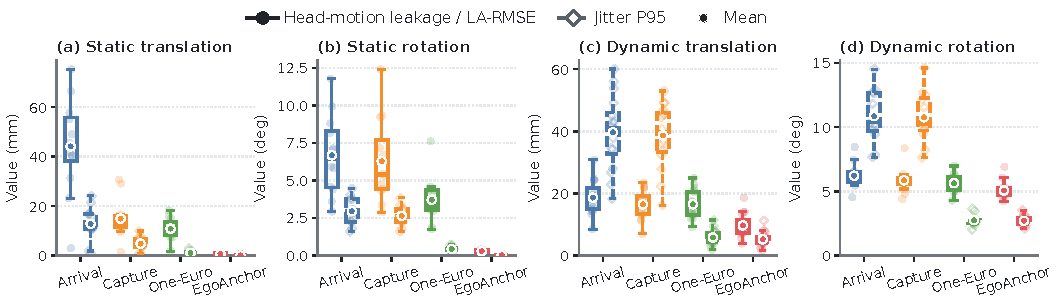
\includegraphics[width=\textwidth]{figures/panels/figure2_exp1_behavior.pdf}
  \caption{Error distributions for the four configurations in Experiment~1. (a,b) Translation and rotation channels while the target is stationary, showing the P95 distributions of head-motion coupling error and static jitter. (c,d) Translation and rotation channels during continuous motion, showing the distributions of LA-RMSE and P95 residual jitter. Each light point denotes one repeated trial. Boxes and center lines show the IQR and median, respectively, and dark points show the mean. Lower values are better for all metrics.}
  \label{fig:exp1-final}
\end{figure*}

\subsubsection{Static Registration}

\begin{table}[t]
\centering
\caption{Static-registration metrics in Experiment~1. Each cell reports the median across repeated trials as translation/rotation; both values are P95 statistics computed within each trial. $\downarrow$ Lower is better; bold indicates the best value in each channel. Distributions appear in Fig.~\ref{fig:exp1-final}(a,b).}
\label{tab:exp1-static}
\begin{tabular}{@{}lccc@{}}
\toprule
Method & \shortstack{Head-motion\\coupling\,$\downarrow$\\mm/$^\circ$} & \shortstack{Registration\\error\,$\downarrow$\\mm/$^\circ$} & \shortstack{Static jitter\,$\downarrow$\\mm/$^\circ$} \\
\midrule
Arrival   & 43.67/6.49 & 44.31/9.65 & 11.70/2.98 \\
Capture   & 13.03/5.40 & 17.54/8.26 & 4.30/2.60 \\
One-Euro  & 10.65/3.29 & 14.00/6.96 & 0.85/0.40 \\
EgoAnchor & \textbf{0.82}/\textbf{0.33} & \textbf{6.60}/\textbf{4.39} & \textbf{0.06}/\textbf{0.03} \\
\bottomrule
\end{tabular}
\end{table}

The active-head-motion test first reveals the temporal mismatch in asynchronous observations. As Table~\ref{tab:exp1-static} shows, Arrival has a head-motion coupling error of 43.67~mm/6.49$^\circ$. Composing the same candidates at image capture time reduces the Capture error to 13.03~mm/5.40$^\circ$. One-Euro yields 10.65~mm/3.29$^\circ$, while the complete EgoAnchor system reaches 0.82~mm/0.33$^\circ$, reductions of approximately 92\% and 90\% relative to One-Euro in the two channels. Absolute registration error follows the same ordering, with EgoAnchor lowest at 6.60~mm/4.39$^\circ$. For static jitter, the two configurations that directly output the latest candidate show marked high-frequency fluctuations. One-Euro reduces the error to 0.85~mm/0.40$^\circ$, while EgoAnchor reaches 0.06~mm/0.03$^\circ$. Fig.~\ref{fig:exp1-final}(a,\,b) further shows the static output distributions of all four configurations.

\subsubsection{Dynamic Following}

\begin{table}[t]
\centering
\caption{Dynamic-following metrics in Experiment~1. Each cell reports the median across repeated trials as translation/rotation; residual jitter is computed within each trial as a P95 statistic. $\downarrow$ Lower is better; bold indicates the best value in each channel. Distributions appear in Fig.~\ref{fig:exp1-final}(c,d).}
\label{tab:exp1-dynamic}
\setlength{\tabcolsep}{2pt}
\begin{tabular}{@{}lcccc@{}}
\toprule
Method & \shortstack{Effective\\latency\,$\downarrow$\\ms} & \shortstack{LA-RMSE\,$\downarrow$\\mm/$^\circ$} & \shortstack{CT-RMSE\,$\downarrow$\\mm/$^\circ$} & \shortstack{Residual\\jitter\,$\downarrow$\\mm/$^\circ$} \\
\midrule
Arrival   & \textbf{202.5}/\textbf{255.0} & 18.57/6.09 & \textbf{84.74}/25.44 & 41.08/10.40 \\
Capture   & 255.0/257.5 & 17.14/5.84 & 103.63/\textbf{25.35} & 39.69/10.26 \\
One-Euro  & 380.0/385.0 & 15.69/5.55 & 117.61/34.10 & 5.25/2.70 \\
EgoAnchor & 360.0/345.0 & \textbf{9.12}/\textbf{4.81} & 125.83/31.88 & \textbf{4.56}/\textbf{2.64} \\
\bottomrule
\end{tabular}
\end{table}

After alignment by the optimal effective latency for each method, LA-RMSE captures the geometric trajectory residual with the overall response lag removed. As Table~\ref{tab:exp1-dynamic} shows, EgoAnchor has an LA-RMSE of 9.12~mm/4.81$^\circ$, approximately 42\% and 13\% lower than the corresponding values of 15.69~mm/5.55$^\circ$ for One-Euro in translation and rotation, respectively. The dynamic residual jitter is 4.56~mm/2.64$^\circ$ for EgoAnchor and 5.25~mm/2.70$^\circ$ for One-Euro. Compared with the stationary condition, the gap in residual jitter narrows, while the LA-RMSE difference is concentrated in translation.

Current-time registration follows a different pattern. The configurations that directly output candidates have lower response latency (202.5/255.0~ms for Arrival). With state estimation and historical interpolation, effective latency is 380.0/385.0~ms for One-Euro and 360.0/345.0~ms for EgoAnchor. Without latency alignment, this lag contributes to instantaneous error: translation CT-RMSE increases from 84.74~mm for Arrival to 125.83~mm for EgoAnchor, whereas the rotation CT-RMSE of EgoAnchor (31.88$^\circ$) is lower than that of One-Euro (34.10$^\circ$). These results show that lower latency-aligned trajectory residuals (LA-RMSE) come with some registration phase lag.

\subsubsection{State-Transition Response}

\begin{table}[t]
\centering
\caption{State-transition response metrics in Experiment~1. Occlusion-recovery error is reported as the median across repeated trials of the within-trial P95 translation/rotation value; motion-response latency is the median scalar shared across channels. $\downarrow$ Lower is better; bold indicates the best value.}
\label{tab:exp1-transition}
\begin{tabular}{@{}lcc@{}}
\toprule
Method & \shortstack{Occlusion\\recovery error\,$\downarrow$\\mm/$^\circ$} & \shortstack{Motion-response\\latency\,$\downarrow$\\ms} \\
\midrule
Arrival   & 18.23/18.39 & \textbf{157.0} \\
Capture   & 16.93/18.38 & 263.8 \\
One-Euro  & 10.41/8.66  & 334.0 \\
EgoAnchor & \textbf{4.85}/\textbf{5.52} & 510.4 \\
\bottomrule
\end{tabular}
\end{table}

Table~\ref{tab:exp1-transition} compares occlusion-recovery error with motion-response latency. During brief complete occlusion and subsequent recovery, occlusion-recovery error decreases from 18.23~mm/18.39$^\circ$ for Arrival and 10.41~mm/8.66$^\circ$ for One-Euro to 4.85~mm/5.52$^\circ$ for EgoAnchor. Relative to One-Euro, EgoAnchor reduces the two channels by approximately 53\% and 36\%. Motion-response latency correspondingly increases from 157.0~ms for Arrival and 334.0~ms for One-Euro to 510.4~ms for EgoAnchor, revealing a tradeoff between accuracy and response speed.

\subsubsection{Qualitative Replay}

\begin{figure}[t]
  \centering
  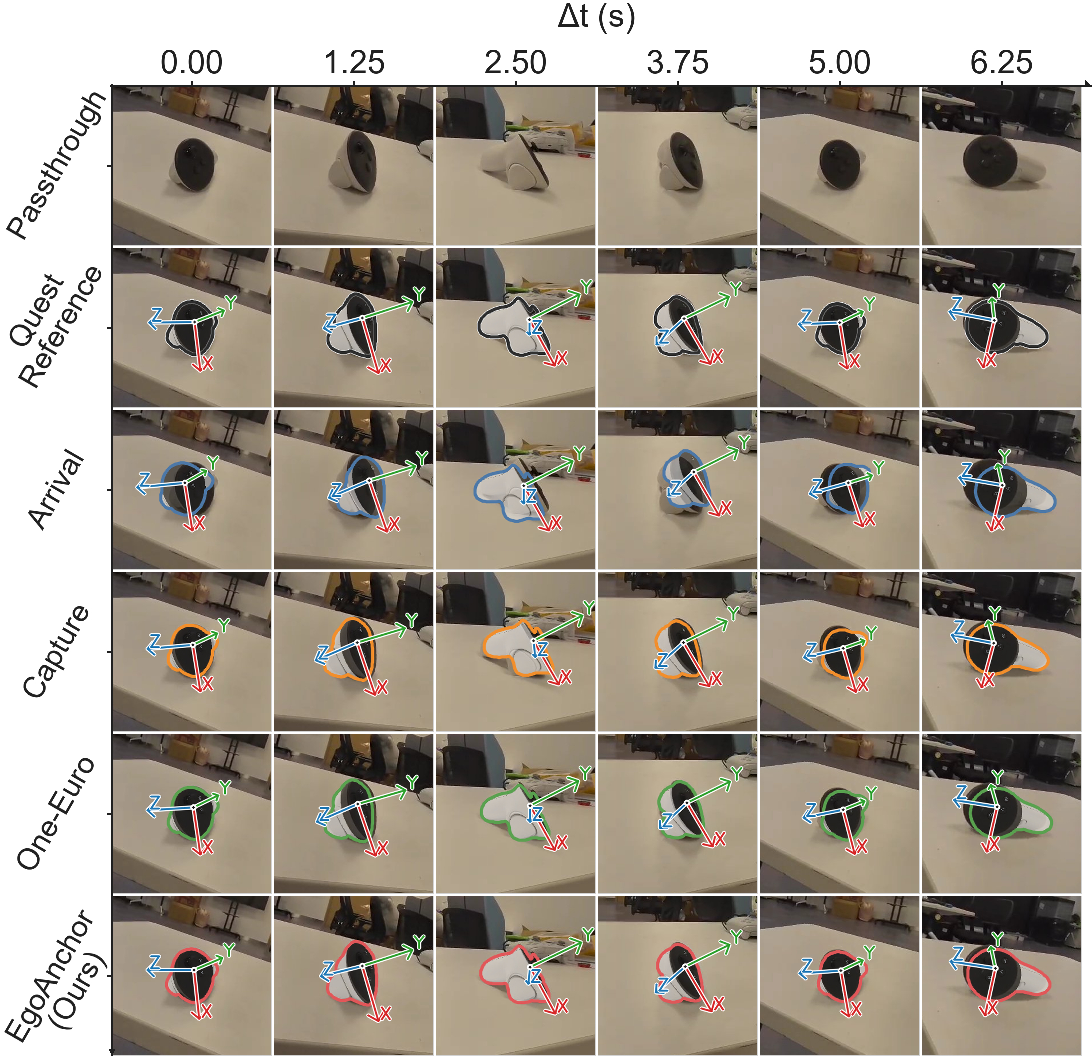
\includegraphics[width=\columnwidth]{figures/replay_grid.pdf}
  \caption{Continuous sequence replay in Experiment~1 ($\Delta t=0$--$6.25\,\mathrm{s}$ at $1.25\,\mathrm{s}$ intervals). The top two rows show the raw passthrough image and Quest platform tracking reference. The bottom four rows show anchor projections from Arrival, Capture, One-Euro, and EgoAnchor at the same capture times. Outlines and local axes indicate the estimated 6-DoF anchors and allow comparison of registration and temporal continuity under head and object motion.}
  \label{fig:exp1-replay}
\end{figure}

Fig.~\ref{fig:exp1-replay} shows how the quantitative differences appear during continuous interaction. Under head motion, Arrival and Capture exhibit clear spatial offsets. One-Euro reduces some of these offsets, while EgoAnchor maintains lower real--virtual alignment error.

\subsection{Experiment 2: Ablation Analysis}

Each ablation in Experiment~2 uses independently collected paired measurements. Each repeated trial is first aggregated within its sequence, after which statistics across repetitions are reported. Brackets indicate bootstrap 95\% confidence intervals, and relative changes are reported as paired ratios.

\begin{figure*}[!t]
  \centering
  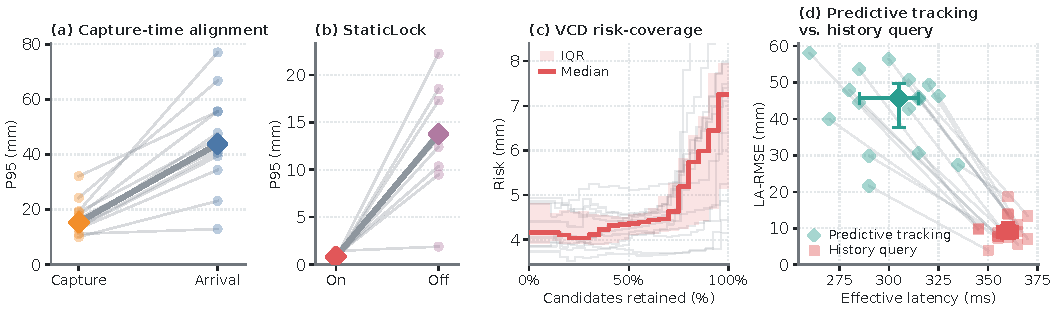
\includegraphics[width=\textwidth]{figures/panels/figure3_exp2_attribution.pdf}
  \caption{Component ablations in Experiment~2. (a) P95 distributions of head-motion coupling error when composing with the camera pose at capture or arrival time. (b) P95 distributions of head-motion coupling error with StaticLock enabled or disabled. (c) VCD risk--coverage curve; thin gray curves show individual repetitions, and the red line and shading show the median and IQR across repetitions. (d) Translation-channel tradeoff between effective latency and LA-RMSE for predictive tracking and history query. In (a), (b), and (d), thin gray lines connect paired measurements; large colored markers and error bars show the median and IQR, respectively.}
  \label{fig:exp2-final}
\end{figure*}

Fig.~\ref{fig:exp2-final}(a,b) evaluates the temporal semantics used for frame composition and the effect of StaticLock. Under active head motion and for the same set of camera-frame pose candidates, composition with the camera pose at image capture time yields a median P95 head-motion coupling error of 15.38~mm. Using the camera pose at candidate-arrival time increases this error to 43.75~mm, with a paired ratio of 2.69 [2.38, 3.00]. Capture-time alignment therefore reduces spatial mismatch caused by head motion. Disabling StaticLock in the complete EgoAnchor system increases P95 head-motion coupling error under stationary conditions from 0.82~mm to 13.73~mm, a paired ratio of 17.06 [13.89, 27.52]. StaticLock thus reduces output fluctuations while the object is stationary.

Fig.~\ref{fig:exp2-final}(c) uses a risk--coverage curve to evaluate the relationship between VCD score and translation error. As candidate admission expands from high-scoring to low-scoring candidates, selective risk generally rises. Under occlusion, the AURC is 4.79 [4.20, 5.13]~mm, and the risk at full coverage is 7.25 [5.15, 7.95]~mm. This trend indicates that VCD captures the relative geometric reliability of pose candidates and provides a useful ranking for candidate selection.

Fig.~\ref{fig:exp2-final}(d) compares predictive tracking and history query in response latency and trajectory fidelity. Predictive tracking has an effective latency of 305.00/250.00~ms, lower than the 360.00/345.00~ms of history query. Its latency-aligned trajectory residual (LA-RMSE), however, is 45.64~mm/12.21$^\circ$, higher than the 8.93~mm/4.70$^\circ$ of history query. Based on paired ratios, the translation and rotation trajectory residuals under prediction are 5.46 [4.02, 5.73] and 2.63 [2.44, 2.78] times those under history query, respectively. Predictive tracking reduces response latency but increases trajectory-estimation error, whereas history query provides higher geometric trajectory fidelity.

\subsection{Experiment 3: User Study}

Fig.~\ref{fig:exp3-subjective} shows paired ratings from the 24 participants. Complete statistics for all 12 outcomes, including medians, Wilcoxon statistics, Holm-adjusted $p$ values, and effect sizes, appear in the supplemental material. The main text focuses on statistically significant or representative results.

\begin{figure*}[!t]
  \centering
  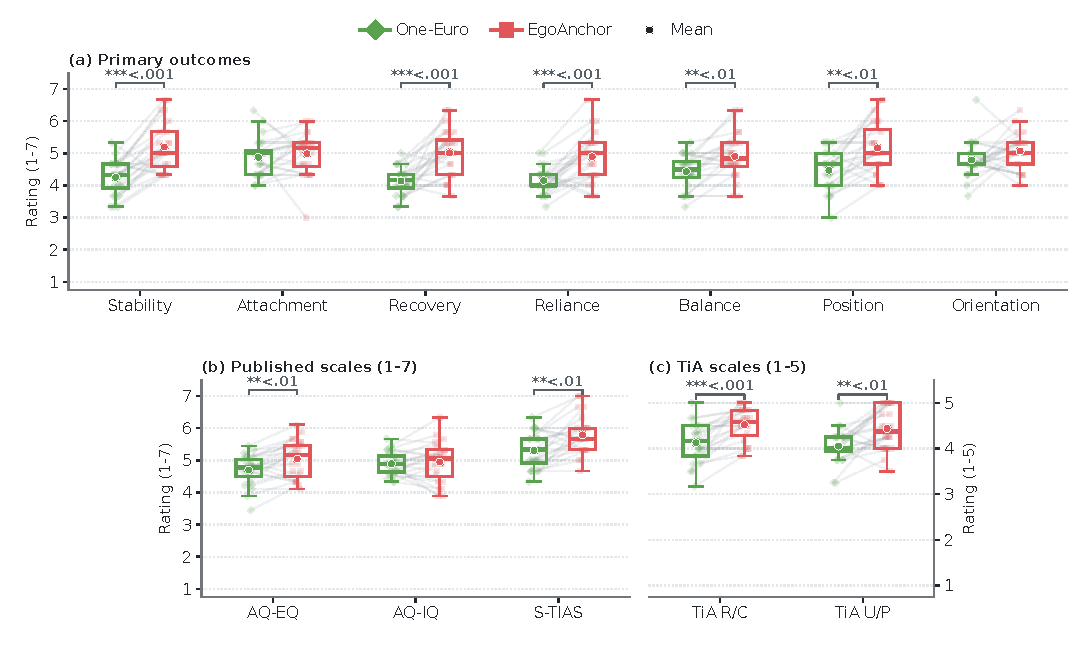
\includegraphics[width=\textwidth]{figures/panels/figure4_exp3_subjective_outcomes.pdf}
  \caption{Within-subject ratings of One-Euro and EgoAnchor from 24 participants. (a) Static stability, attachment during motion, pose consistency, and recovery consistency. (b) Positional correctness, willingness to rely on the system, and the stability--responsiveness tradeoff. (c) AQ-EQ, AQ-IQ, and S-TIAS. (d) TiA Reliability/Competence (R/C) and Understanding/Predictability (U/P). Each anchoring-item score and each AQ subscale score is first averaged across the three objects. Panels (a)--(c) use seven-point scales, and (d) uses five-point scales. Light points and gray lines show individual paired ratings; boxes, horizontal lines, and black points show the IQR, median, and mean. Asterisks denote Holm-adjusted significance levels ($^*p_{\mathrm{adj}}<.05$, $^{**}p_{\mathrm{adj}}<.01$, $^{***}p_{\mathrm{adj}}<.001$).}
  \label{fig:exp3-subjective}
\end{figure*}

\subsubsection{Object-Anchoring Experience}

\textbf{Stationary and recovery phases.}
The largest effects among the seven items occur during the stationary and recovery phases. Under static observation, EgoAnchor has a median rating of 5.00 [4.58, 5.67], higher than the rating of 4.33 [3.92, 4.67] for One-Euro ($W=13.5$, $p_{\mathrm{adj}}<.001$, $r_{\mathrm{rb}}=.90$). After the occluder is removed, recovery consistency is 5.00 [4.33, 5.42] for EgoAnchor and 4.17 [3.92, 4.33] for One-Euro. This difference has the largest effect size among the seven items ($W=6$, $p_{\mathrm{adj}}<.001$, $r_{\mathrm{rb}}=.95$).

\textbf{Continuous-motion phase.}
During continuous object manipulation, the perceived difference between the systems narrows markedly. Attachment-during-motion ratings are similar for EgoAnchor (5.17 [4.58, 5.33]) and One-Euro (5.00 [4.33, 5.08]). Pose-consistency ratings are 5.00 [4.67, 5.33] for EgoAnchor and 4.67 [4.67, 5.00] for One-Euro. Neither difference is statistically significant after Holm correction (attachment: $W=67.5$, $p_{\mathrm{adj}}=.267$, $r_{\mathrm{rb}}=.29$; consistency: $W=81$, $p_{\mathrm{adj}}=.162$, $r_{\mathrm{rb}}=.41$).

\textbf{Overall anchoring judgments.}
All three overall measures show statistically significant differences in favor of EgoAnchor. Positional correctness is 5.00 [4.67, 5.75] for EgoAnchor and 4.67 [4.00, 5.00] for One-Euro ($W=16$, $p_{\mathrm{adj}}=.001$, $r_{\mathrm{rb}}=.85$). Willingness to rely on the system is 5.00 [4.33, 5.33] for EgoAnchor and 4.00 [4.00, 4.33] for One-Euro ($W=16.5$, $p_{\mathrm{adj}}<.001$, $r_{\mathrm{rb}}=.87$). Ratings of the stability--responsiveness tradeoff are 4.83 [4.58, 5.33] for EgoAnchor and 4.50 [4.25, 4.75] for One-Euro ($W=6$, $p_{\mathrm{adj}}=.003$, $r_{\mathrm{rb}}=.90$).

\subsubsection{Augmentation Quality and Trust}

\textbf{Augmentation quality.}
The AQ analysis indicates that the system difference lies mainly in perceived real--virtual integration (AQ-EQ), rather than dynamic interaction quality (AQ-IQ). The Embedding Quality score is 5.17 [4.50, 5.47] for EgoAnchor, higher than the score of 4.78 [4.50, 5.03] for One-Euro ($W=32$, $p_{\mathrm{adj}}=.004$, $r_{\mathrm{rb}}=.75$). The difference in Interaction Quality does not reach the adjusted significance level: 5.06 [4.50, 5.33] for EgoAnchor and 4.89 [4.64, 5.14] for One-Euro ($W=102.5$, $p_{\mathrm{adj}}=.446$, $r_{\mathrm{rb}}=.19$).

\textbf{User trust.}
EgoAnchor receives higher ratings on all three trust measures. TiA Reliability/Competence has the largest effect ($W=0$, $p_{\mathrm{adj}}<.001$, $r_{\mathrm{rb}}=1.00$): 4.58 [4.29, 4.83] for EgoAnchor and 4.17 [3.83, 4.50] for One-Euro. For Understanding/Predictability, EgoAnchor scores 4.38 [4.00, 5.00] and One-Euro 4.00 [3.94, 4.25] ($W=32$, $p_{\mathrm{adj}}=.004$, $r_{\mathrm{rb}}=.75$). Overall S-TIAS trust ratings also differ significantly: 5.67 [5.33, 6.00] for EgoAnchor and 5.33 [4.92, 5.67] for One-Euro ($W=22.5$, $p_{\mathrm{adj}}=.004$, $r_{\mathrm{rb}}=.79$).

Scale-reliability analysis shows low internal consistency for AQ Interaction Quality ($\alpha=.504$) and TiA Understanding/Predictability ($\alpha=.565$) under One-Euro. S-TIAS also has $\alpha<.70$ under both methods ($.672$ for One-Euro and $.697$ for EgoAnchor). These scale-level differences should therefore be interpreted cautiously; complete reliability coefficients appear in the supplemental material.

\textbf{Overall choices.}
In the blinded overall preference question, 62.5\% (15/24) of participants prefer EgoAnchor, four prefer One-Euro, and five report no clear preference. When directly asked which method they trust, 18 choose EgoAnchor, one chooses One-Euro, and five consider them equivalent. Median preference strength is 4.00 [3.00, 5.00], and median confidence in distinguishing the methods is 6.00 [5.00, 7.00]. Only three participants reported mild discomfort during the study, and none withdrew.

\section{Discussion}\label{sec:discussion}

\subsection{Technical Implications}

Across the controlled evaluation and user study, the clearest performance gains come from explicitly restoring the temporal semantics of image capture and modeling the stationary state, rather than relying only on frame-to-frame adaptive smoothing. VCD provides an effective reliability ranking for pose candidates, while history query reduces geometric trajectory residuals at the cost of response lag. These objective differences align with the higher participant ratings of EgoAnchor for real--virtual integration, positional correctness, willingness to rely on the system, and interaction trust. For egocentric dynamic anchoring, a practical system must jointly organize pose geometry, capture timestamps, observation reliability, and asynchronous transmission into an object state that supports continuous application-level binding.

EgoAnchor presents a clear system tradeoff. It provides higher static stability, occlusion-recovery accuracy, and geometric trajectory fidelity, but has longer motion-response latency. During continuous motion, its instantaneous translation error (CT-RMSE) exceeds that of baselines that directly output candidates. The user study shows the same pattern: the benefits of EgoAnchor concentrate on static observation, occlusion recovery, and overall trust, whereas the two methods do not differ significantly in subjective ratings during continuous manipulation. Tasks that prioritize spatial alignment, such as physical annotation, assembly guidance, and state monitoring, can favor stability and geometric fidelity. Highly dynamic, latency-sensitive interactions require further reduction of response latency.

\subsection{Limitations and Future Work}

\textbf{Objects and 3D models.}
EgoAnchor currently targets everyday objects with known rigid 3D models. Its anchoring performance depends on target observability and the quality of the model prior. Severe line-of-sight occlusion, weakly textured surfaces, highly reflective or translucent materials, and stereo depth failures all affect the accuracy of segmentation masks and pose verification. Deformable objects fall outside the scope of our rigid-object model. In addition, because the same 3D model is used for both pose estimation and VCD verification, geometric or scale errors in the model directly introduce systematic error. Future work can explore lightweight online geometric calibration and automated model-generation pipelines.

\textbf{Evaluation reference and cross-platform comparison.}
Our controlled benchmark using a platform-tracked controller reference is limited to Meta Quest 3 and does not provide a direct 6-DoF comparison across headset platforms. Platforms differ in their requirements for model origin, axis conventions, scale, and preprocessing, so output poses are defined in different local object frames. Their sensor configurations, clock synchronization, and tracking interfaces also differ. Although the Quest 3 controller provides an accurate synchronized reference, it still relies on native visual--inertial estimation of the platform rather than absolute ground truth. Future benchmarks can calibrate a common object coordinate frame and use optical motion capture or a high-precision robotic arm for stricter cross-platform evaluation.

\textbf{Deployment and evaluation benchmark.}
The current system relies on an external high-performance GPU workstation for perception inference, and network communication and heterogeneous computing introduce inherent latency. Model quantization, distillation, and mobile NPU acceleration could enable a lightweight on-headset perception pipeline, reducing end-to-end latency and improving support for fast dynamic manipulation. The controlled benchmark uses the official controller to obtain an accurate tracking reference, while the user study uses three rigid objects to balance object diversity and study duration. Future work can apply the three metric groups---static registration, dynamic following, and state-transition response---to more object classes and heterogeneous headsets, further developing a standardized benchmark for dynamic object anchoring~\cite{cheng2024tracking,hu2024applemeta,hu2025xrrealitycheck}.

\section{Conclusion}\label{sec:conclusion}

We present EgoAnchor, an egocentric system for zero-shot dynamic object anchoring in passthrough mixed reality. It transforms asynchronous camera-frame observations into world-frame states at image capture time and maintains a reliable object state for the rendering pipeline. This runtime process converts discrete, low-rate visual estimates into continuous, stable object anchors with occlusion recovery. Controlled benchmarks and ablations show that EgoAnchor reduces static registration error, occlusion-recovery error, and geometric trajectory residuals relative to the baselines, but increases motion-response latency. A within-subject study with 24 participants further shows higher ratings for real--virtual integration, interaction trust, and willingness to rely on the system.

Transforming visually estimated poses into usable object-level spatial anchors requires more than single-frame pose accuracy; it requires systematic runtime modeling of temporal semantics, perceptual uncertainty, and the state lifecycle. With continued advances in open-vocabulary foundation models, rapid 3D generation, and mobile computing, coordinated perception--runtime architectures may enable high-fidelity dynamic anchoring for a broader range of everyday objects and mixed-reality interactions.

\acknowledgments{
  This work is supported by the National Natural Science Foundation of China (No. 62377004). OpenAI ChatGPT was used only to assist with English translation and language editing. The authors reviewed and verified all revisions.
}

\bibliographystyle{abbrv-doi-hyperref-narrow}
\bibliography{egoanchor_cn_refs}

\end{document}
